\documentclass[../notes.tex]{subfiles}

\pagestyle{main}
\renewcommand{\chaptermark}[1]{\markboth{\chaptername\ \thechapter\ (#1)}{}}
\stepcounter{chapter}

\begin{document}




\chapter{DNA}
\section{DNA Synthesis and Transcription}
\begin{itemize}
    \item \marginnote{10/4:}DNA binding proteins.
    \begin{itemize}
        \item Interact with major grooves of DNA to achieve sequence specificity.
        \item Example: Transcription factors that have to turn a gene on or off.
        \item Such proteins often do this with two primary motifs: The leucine zipper and the zinc finger.
        \begin{itemize}
            \item Leucine zipper: Less programmable.
            \item Zinc finger: More programmable. Contains 1+ zinc ion coordinated by cysteine and histidine. One zinc finger interacts with three base pairs.
        \end{itemize}
        \item With the scale of our genome, you typically need a sequence of 15-18 base pairs to achieve specificity. That's 5-6 zinc fingers.
        \item When they were discovered, zinc fingers were thought to be a possibility for genome editing.
    \end{itemize}
    \item DNA structure and binding modes.
    \begin{itemize}
        \item DNA binding proteins may also interact with the minor group (to achieve some specificity), electrostatically with the phosphate backbone (usually not sequence-specific), and intercalation (a flat molecule splits two base pairs a bit and inserts itself in).
    \end{itemize}
    \item Minor groove: Deep and narrow.
    \begin{itemize}
        \item Minor groove binding can involve electrostatics, hydrophobic burial, and hydrogen bonding.
        \item Minor groove binding can be site specific. There are some features you can take advantage of, e.g., being flat and flexible.
    \end{itemize}
    \item Pyrrole-Imidazole-Hydroxypyrrole (Py/Im/Hp) Polyamides.
    \begin{itemize}
        \item Pioneered by the Dervan lab at CalTech.
        \item Minor-groove binding polyamides consisting of three aromatic ring amino acids.
        \item Flexible because of the amides.
        \item Eight-ring pyrrole-imidazole polyamides achieve affinities and specificities comparable to DNA-binding proteins.
        \item Cell-permeable molecules for gene-specific regulation \emph{in vivo}.
        \item Still not specific enough, though.
    \end{itemize}
    \item Minor groove-binding small molecules.
    \begin{itemize}
        \item Examples (not testable material): Hoechst 33258, DAPI, Distamycin, and Berenil.
        \begin{itemize}
            \item Distamycin in the minor groove. Distamycin is an antibiotic and it fits very well into the minor groove. Preference for A/T sequences.
            \item Hoechst 33258 in the minor groove. Also fits very well; uset to some extent to dye DNA, but more often in flow cytometry.
        \end{itemize}
        \item Common features (testable material):
        \begin{itemize}
            \item Flat (to slip into the minor groove).
            \item Small linked aromatic ring systems (to allow ring systems to make local adjustments).
            \item Curved (to match curvature of the minor groove).
            \item Positively charged (to interact with the phosphates).
            \item H-bond donors on concave face (to H-bond with acceptors on base pairs).
        \end{itemize}
    \end{itemize}
    \item Phosphate backbone binding.
    \begin{itemize}
        \item Driven by electrostatics.
        \begin{itemize}
            \item Ligands that bind this way are always cationic, binding depends strongly on salt concentration.
            \item Ions (\ce{Na+}, \ce{Mg^2+}, etc.)
        \end{itemize}
        \item Example: Biogenic polyamines (involved in a lot of biological processes).
        \begin{itemize}
            \item For example, putrescine is a positively charged polyamine. It is responsible for bad breath!
        \end{itemize}
        \item \textbf{Transfaction reagents} wrap around DNA and neutralize some of its negative charge to help it get into cells.
    \end{itemize}
    \item Intercalators.
    \begin{itemize}
        \item Example: Ethidium bromide (a toxic molecule used to stain DNA).
        \item Features in common:
        \begin{itemize}
            \item Extended aromatic systems (to provide extensive overlap with base pairs).
            \item Electron deficient (to complement regions of high electron density in base pairs).
        \end{itemize}
    \end{itemize}
    \item Intercalation requires structural rearrangement.
    \begin{itemize}
        \item The intercalator does disturb DNA structure a bit as it pushes base pairs farther apart, causing buckling in adjacent base pairs and a tilt in the helical axis.
        \item Because of this, intercalators can alter DNA replication.
    \end{itemize}
    \item Ethidium bromide as a DNA dye.
    \begin{itemize}
        \item Biochemical analysis of DNA (gel electrophoresis).
        \begin{itemize}
            \item Agarose is used for DNA strands over 300 bp. Bands greater than 100,000 bp are not resolved.
            \item Concentration of agarose can be increased to create a denser matrix, or decreased to create a less dense matrix.
            \item Larger molecules need a less dense matrix.
            \item Because DNA is negatively charged, it migrates to the cathode (+) of the electrophoresis system.
        \end{itemize}
        \item Ethidium bromide is toxic: It can act as a mutagen because it intercalates double-stranded DNA and, as mentioned, affects replication.
        \begin{itemize}
            \item If you add too much ethidium bromide into your PCR, it may not work (the polymerase may not be able to overcome it).
        \end{itemize}
        \item Safer options are offered by many biotech companies: sybr-green, sybr-gold, etc.
        \begin{itemize}
            \item Tang isn't sure how much safer these actually are.
            \item The common design is bigger molecules: Will still intercalate DNA, but will not penetrate the skin as easily.
        \end{itemize}
    \end{itemize}
    \item Summary.
    \begin{itemize}
        \item Several forms of DNA/RNA (most important ones: A-RNA and B-DNA).
        \item Unusual forms may also play an important role (e.g., G-quadruplex and tRNA).
        \begin{itemize}
            \item 
        \end{itemize}
        \item Molecules that interact with the DNA.
        \begin{itemize}
            \item Major grove interactions are sequence specific.
            \item Minor grove interactions can be sequence specific.
            \item Phosphate backbone/intercalation interactions are (typically) not sequence specific.
        \end{itemize}
    \end{itemize}
    \item This is the end of the previous lecture's slides.
    \item Now: Replication, transcription, translation, and nucleic acid catalysis.
    \item Overview.
    \begin{itemize}
        \item DNA replication in cells: DNA-templated synthesis of DNA.
        \item DNA repair in cells: Enzymatic repair of DNA mutations
        \item DNA transcription in cells: DNA-templated synthesis of RNA.
        \item Translation: Nucleic acid catalysis (difficult) and RNA-templated synthesis of proteins.
    \end{itemize}
    \item If you find the early topics above difficult, review the relevant sections of \textcite{bib:Lehninger}.
    \item DNA is synthesized/replicated by DNA polymerase.
    \begin{figure}[h!]
        \centering
        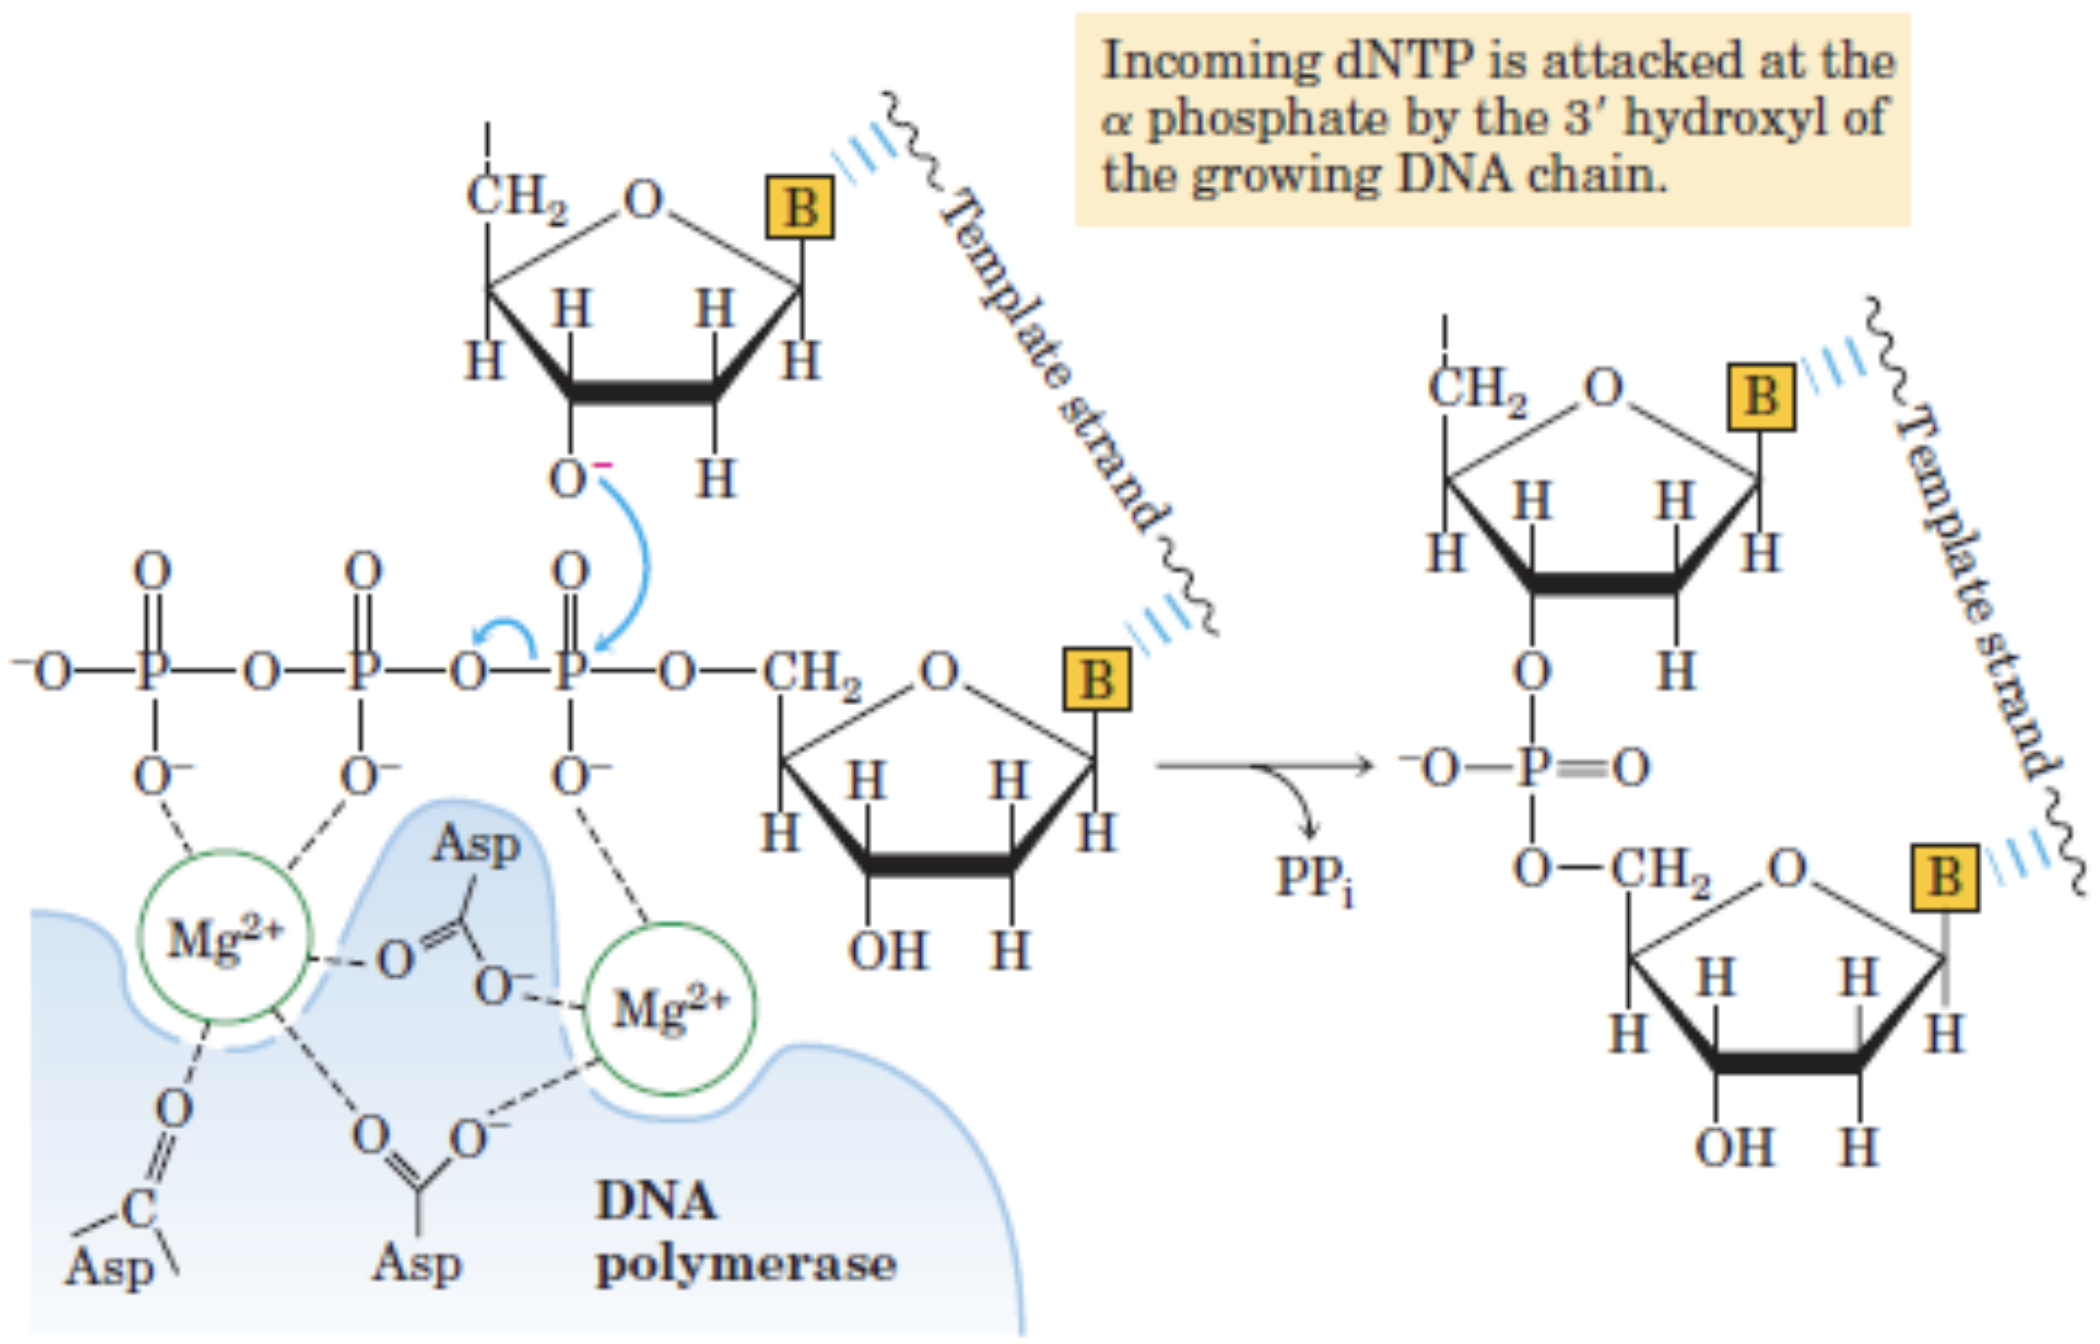
\includegraphics[width=0.6\linewidth]{../ExtFiles/DNASynMech.png}
        \caption{Mechanism of DNA synthesis.}
        \label{fig:DNASynMech}
    \end{figure}
    \begin{itemize}
        \item DNA polymerases require three components: A template, a primer, and dNTPs\footnote{Deoxynucleoside triphosphate} (N = A, T, G, or C).
        \item Mechanism: The 3' hydroxyl of the growing DNA chain attacks the $\alpha$ phosphate of the incoming dNTP via nucleophilic acyl substitution.
        \begin{itemize}
            \item Most textbooks will draw the electron pushing as a substitution reaction, but in reality, the double bond gets resolved, and then kicks back down to get rid of the $\beta$ and $\gamma$ phosphates.
            \item Energetically driven by the BDE of the dNTP, so as long as dNTP is abundant, the reaction can proceed.
        \end{itemize}
        \item In bacteria, this process can occur at a rate of 1000 bp/second.
        \begin{itemize}
            \item Our cells are slower.
        \end{itemize}
        \item Notice the presence here of magnesium (partially coordinated to aspartic acid) catalyzing the reaction as part of DNA polymerase.
        \begin{itemize}
            \item One \ce{Mg^2+} coordinates with the $\beta$ and $\gamma$ phosphates to stabilize them.
            \item The other coordinates with the $\alpha$ phosphate to stabilize the highly negatively charged nucleophilic acyl substitution intermediate.
        \end{itemize}
        \item DNA replication in \emph{E. coli} is highly accurate (error rate \numrange{e-9}{e-10}).
        \begin{itemize}
            \item Two reasons: Templated synthesis (error rate of \numrange{e-4}{e-5} \emph{in vitro}) and error correction mechanisms.
        \end{itemize}
        \item Templated synthesis is equivalent to having a 99.999\% yield in an organic reaction (which never happens).
        \item One error-correction mechanism bridging the gap from \num{e-5} to \num{e-10}: DNA polymerase "proofreads" even as it synthesizes DNA.
        \item Example procedure:
        \begin{itemize}
            \item Let C* be a rare tautomer of cytosine that pairs with A and is incorporated into the growing strand.
            \item Before the polymerase moves on, the C* reconverts to C and is now mispaired.
            \item The mispaired 3'-OH end of the growing strand blocks further elongation. DNA polymerase slides back to position the mispaired base in the $3'\to 5'$ exonuclease active site.
            \item The mispaired nucleotide is removed.
            \item DNA polymerase slides forward and resumes its polymerization activity.
        \end{itemize}
        \item Not every polymerase has this feature, but most high-fidelity ones do.
    \end{itemize}
    \item DNA replication in cells.
    \begin{itemize}
        \item DNA replication is semiconservative.
        \begin{itemize}
            \item Meselson-Stahl experiment, "the most beautiful experiment in biology."
        \end{itemize}
        \item DNA replication begins at an \textbf{origin} and proceeds \textbf{bidirectionally}.
        \item Bacterial chromosomes have a single point of origin; most other cells have multiple such points.
    \end{itemize}
    \item DNA replication requires many enzymes and protein cofactors.
    \begin{itemize}
        \item DNA replication in cells requires much more than solely polymerases.
        \item DNA replication in \emph{E. coli} requires 20 or more different enzymes and proteins, each performing a specific task.
        \item DNA replicase system (replisome): The entire complex is required for DNA replication.
        % \item Key proteins of the \emph{E. coli} replisome.
        % \begin{itemize}
        %     \item SSB: Single-stranded DNA binding protein. Stabilizes the exposed single stranded parts of DNA as it is unwound and before its complement is synthesized.
        %     \item Helicase: Unwinds DNA; continuously expands the origin.
        %     \item Primase: Synthesizes a primer. Regardless of whether it's DNA- or RNA-templated synthesis, it's always primed.
        %     \item DNA polymerase vs. ligase: DNA polymerase is the main one; Ligase bridges the lagging strands together.
        % \end{itemize}
    \end{itemize}
    \item Three identifiable phases of DNA replication in \emph{E. coli}.
    \begin{enumerate}
        \item Initiation.
        \begin{itemize}
            \item Five repeats of 9 bp (R sites) for DnaA binding; A = T rich DNA unwinding element (DUE).
            \item DnaA binding, DUE denaturing, DnaB helicase loading, then ready for the next phase.
            \item Initiation is the only phase of DNA replication that is known to be precisely regulated (replication occurs only once in each cell cycle). You don't want the daughter cells to have multiple unneeded copies of the genome.
        \end{itemize}
        \item Elongation.
        \begin{itemize}
            \item Single-stranded DNA-binding protein (SSB) stabilizes the regions denatured by helicase.
            \item Two distinct but related operations: Leading strand synthesis and lagging strand synthesis.
            \item Lagging strand synthesis requires RNA primers (synthesized by primase) to form Okazaki fragments.
            \begin{itemize}
                \item Regardless of whether it's DNA- or RNA-templated synthesis, it's always primed.
            \end{itemize}
            \item After completion of an Okazaki fragment, RNA primer is removed and replaced with DNA by DNA polymerase I, and the remaining nick is sealed by DNA ligase.
        \end{itemize}
        \item Termination.
        \begin{itemize}
            \item Ter sequences: Trap for the bidirectional replication of DNA by forming Tus-Ter complex --- prevent overreplication by one replication folk when the other folk is abnormally delayed or halted.
            \item \textbf{Catenane} formation: Bidirectional replication of DNA meets at the end.
            \item DNA topoisomerase IV: Separate the catenated chromosomes into normal chromosomes for the daughter cells.
        \end{itemize}
    \end{enumerate}
    \item \textbf{Catenane}: A mechanically interlocked molecular architecture consisting of two or more interlocked macrocycles\footnote{Recall the discussion of this in \emph{The Knot Book}!}.
    \item We don't have to remember every protein; Tang just wants to show us.
    \begin{itemize}
        \item Note that the ones that she did show us, though, are all involved in elongation; initiation and termination require additional proteins.
        \item Also, new proteins are still being discovered.
        \item DNA replication in eukaryotic cells is both similar and more complex than in \emph{E. coli}.
    \end{itemize}
    \item Mutations happen constantly in DNA.
    \begin{itemize}
        \item A race between mutation and repair.
        \item Why mutations don't generally affect us: Mutations could occur in DNA that is not used in a given cell (most DNA in any given cell is dormant), the cell could die, etc. Also, only 1\% of our genome is protein-coding. And most amino acids in our proteins are not fully \textbf{conservative}. Significant ones are very rare (and usually lead to apoptosis anyway, so no problem).
        \item Transition (purine to purine, or pyrimidine to pyrimidine), transversion (purine to pyrimidine or vice versa), and frameshift (insertion/deletion by $3n\pm 1$) mutations.
        \begin{itemize}
            \item Frameshift typically corresponds to early stop codon.
        \end{itemize}
        \item Mutation locations and effects.
        \begin{itemize}
            \item Promoter: Reduced or increased gene expression.
            \item Regulatory sequence: Alteration of regulation of gene expression.
            \item $3'$ of protein-coding region: Defective transcription termination or alternation of mRNA stability.
            \item Certain locations within intron: Defective mRNA splicing.
            \item Origin of DNA replication: Defect in initiation of DNA replication.
        \end{itemize}
        \item Many disease-causing mutations in humans are non-coding.
        \item Mutations in one place can interact with other base pairs a few away because they may be close in the 3D structure of DNA. Tang studies this and other noncoding mutations.
    \end{itemize}
    \item \textbf{Conservative} (amino acid): An amino acid in a protein, the identity of which is critical to the form and/or function of the full protein.
    \item The causes of DNA mutations in cells.
    \begin{itemize}
        \item Natural mismatching and tautomerization --- know this!
        \begin{itemize}
            \item Natural mismatching-induced mutation: \numrange{e-9}{e-10}.
            \item Tautomerization ($<0.01\%$ frequency): Mutation if the rare tautomer is paired during DNA replication.
        \end{itemize}
        \item Deamination of exocyclic amines\footnote{Literally: Getting rid of the amine group which lies outside the ring and replacing it with a carbonyl group.} (C, A, G) --- know this!
        \begin{itemize}
            \item Adenine to hypoxanthine.
            \item Guanine to xanthine.
            \item Cytosine to uracil (500 times per day per genome, which is a significant amount). Hence T in DNA but U in RNA.
            \item Cells that are uracil N-glycosylase deficient (ung\textsuperscript{-}) show a higher rate of transitions.
            \item Note: Deamination of A is more common in single-stranded DNA, but deamination of C is exponentially more common in double-stranded DNA.
        \end{itemize}
        \item Depurination (A, G).
        \begin{itemize}
            \item Protonation of purines can lead to cleavage of the glycosyl bond (creating an abasic site).
            \item Abasic sites undergo a retro-Michael-like reaction leading to a phosphodiester bond cleavage. $t_{1/2}\approx\SI{400}{\hour}$ at $37^\circ\text{C},\ \pH=7$.
            \item Mammalian cells can lose as many as 10,000 purines per cell per generation ($k=\num{3e-11}$ per second at $37^\circ\text{C},\ \pH=7$).
            \item Depyrimidination occurs 20 times slower.
        \end{itemize}
        \item Oxidants, radicals, radiations.
        \item Chemicals: Alkylating reagents, nucleophiles, crosslinking reagents, and intercalating reagents.
    \end{itemize}
    \item The reactions of OChem III are not the focus of this course! Tang may occasionally reference such content, but it will be minor and not (directly) tested.
    \item It may seem like our DNA lives a hard life, but in practice, our genome is very stable.
    \item Four strategies of DNA repair in cells.
    \begin{figure}[H]
        \centering
        \begin{subfigure}[b]{0.35\linewidth}
            \centering
            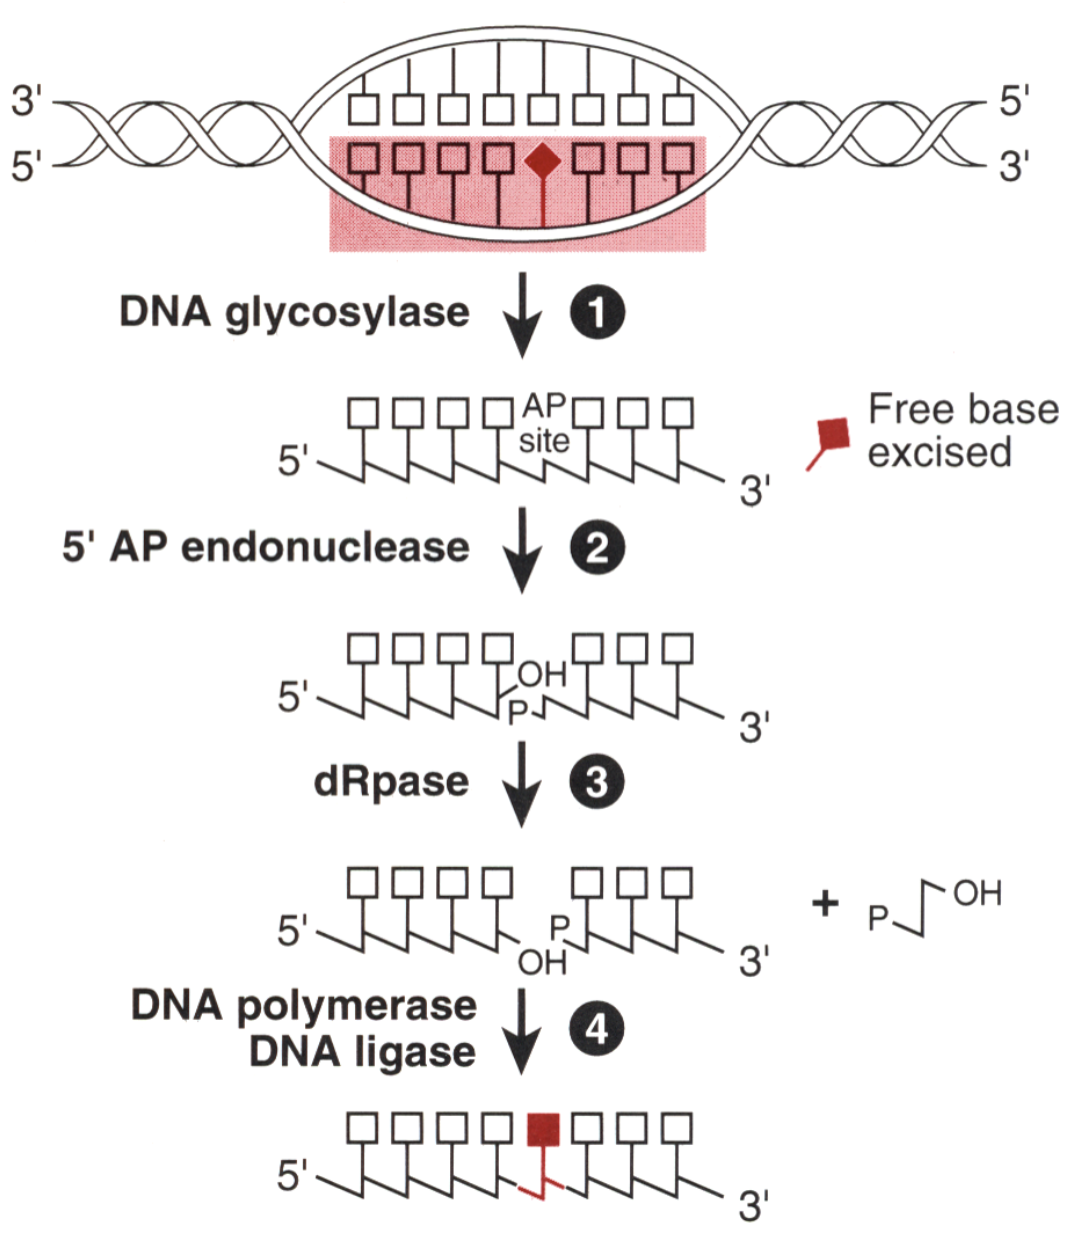
\includegraphics[width=0.98\linewidth]{../ExtFiles/DNARepaira.png}
            \caption{Base excision repair.}
            \label{fig:DNARepaira}
        \end{subfigure}
        \begin{subfigure}[b]{0.63\linewidth}
            \centering
            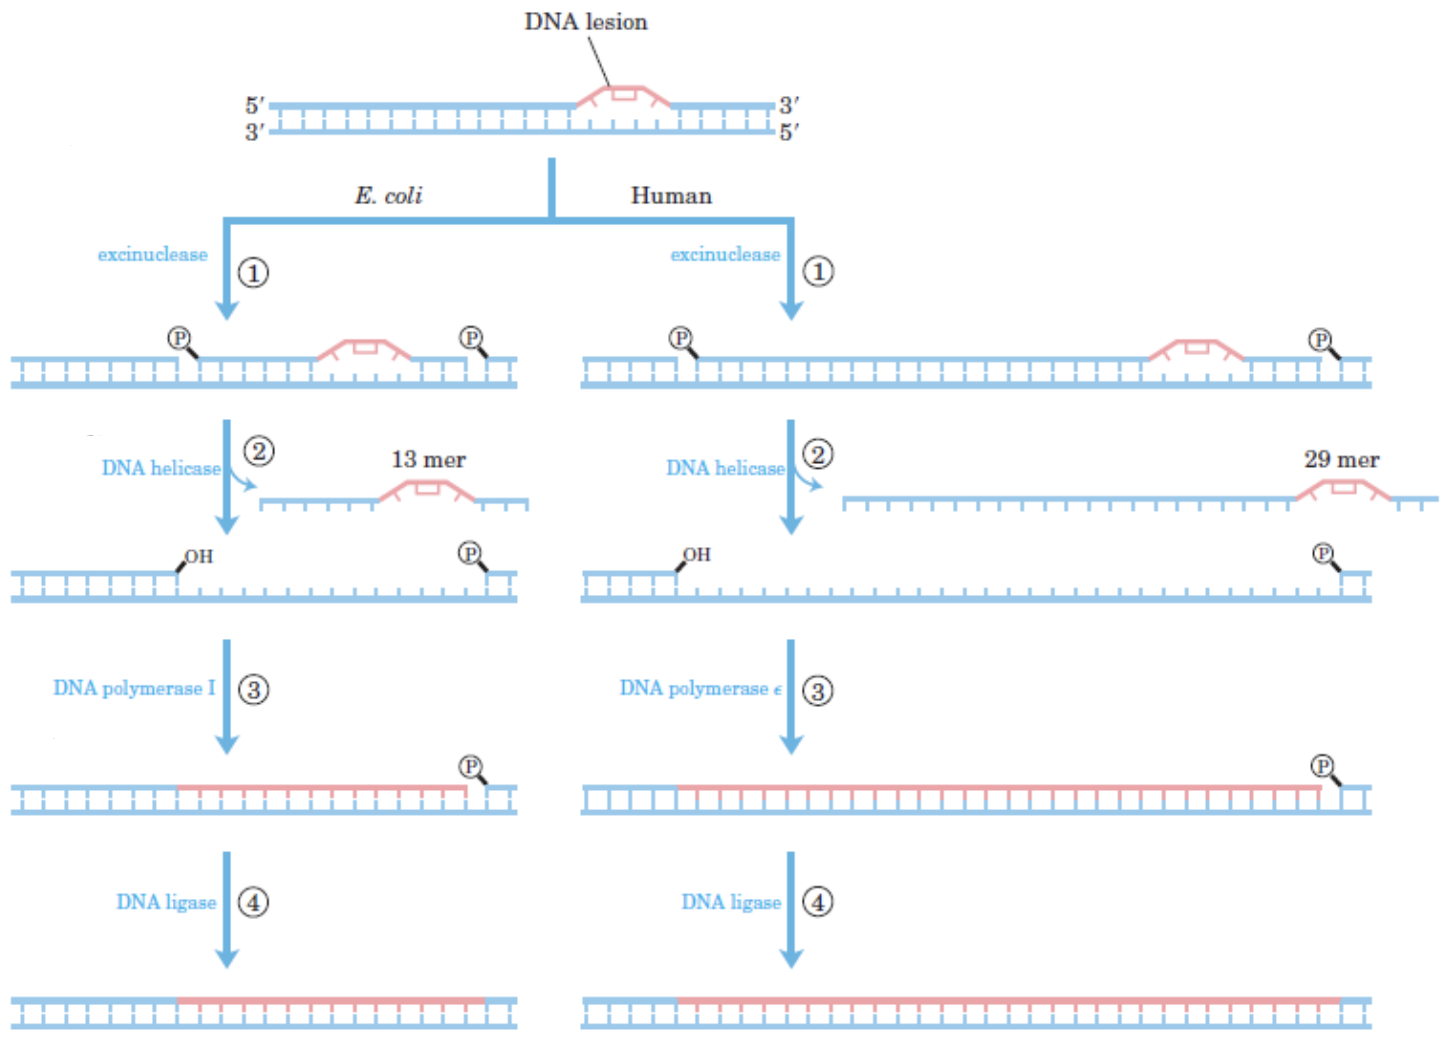
\includegraphics[width=0.9\linewidth]{../ExtFiles/DNARepairb.png}
            \caption{Nucleotide excision repair.}
            \label{fig:DNARepairb}
        \end{subfigure}
    \end{figure}
    \begin{figure}[H]
        \ContinuedFloat
        \centering
        \begin{subfigure}[b]{0.8\linewidth}
            \centering
            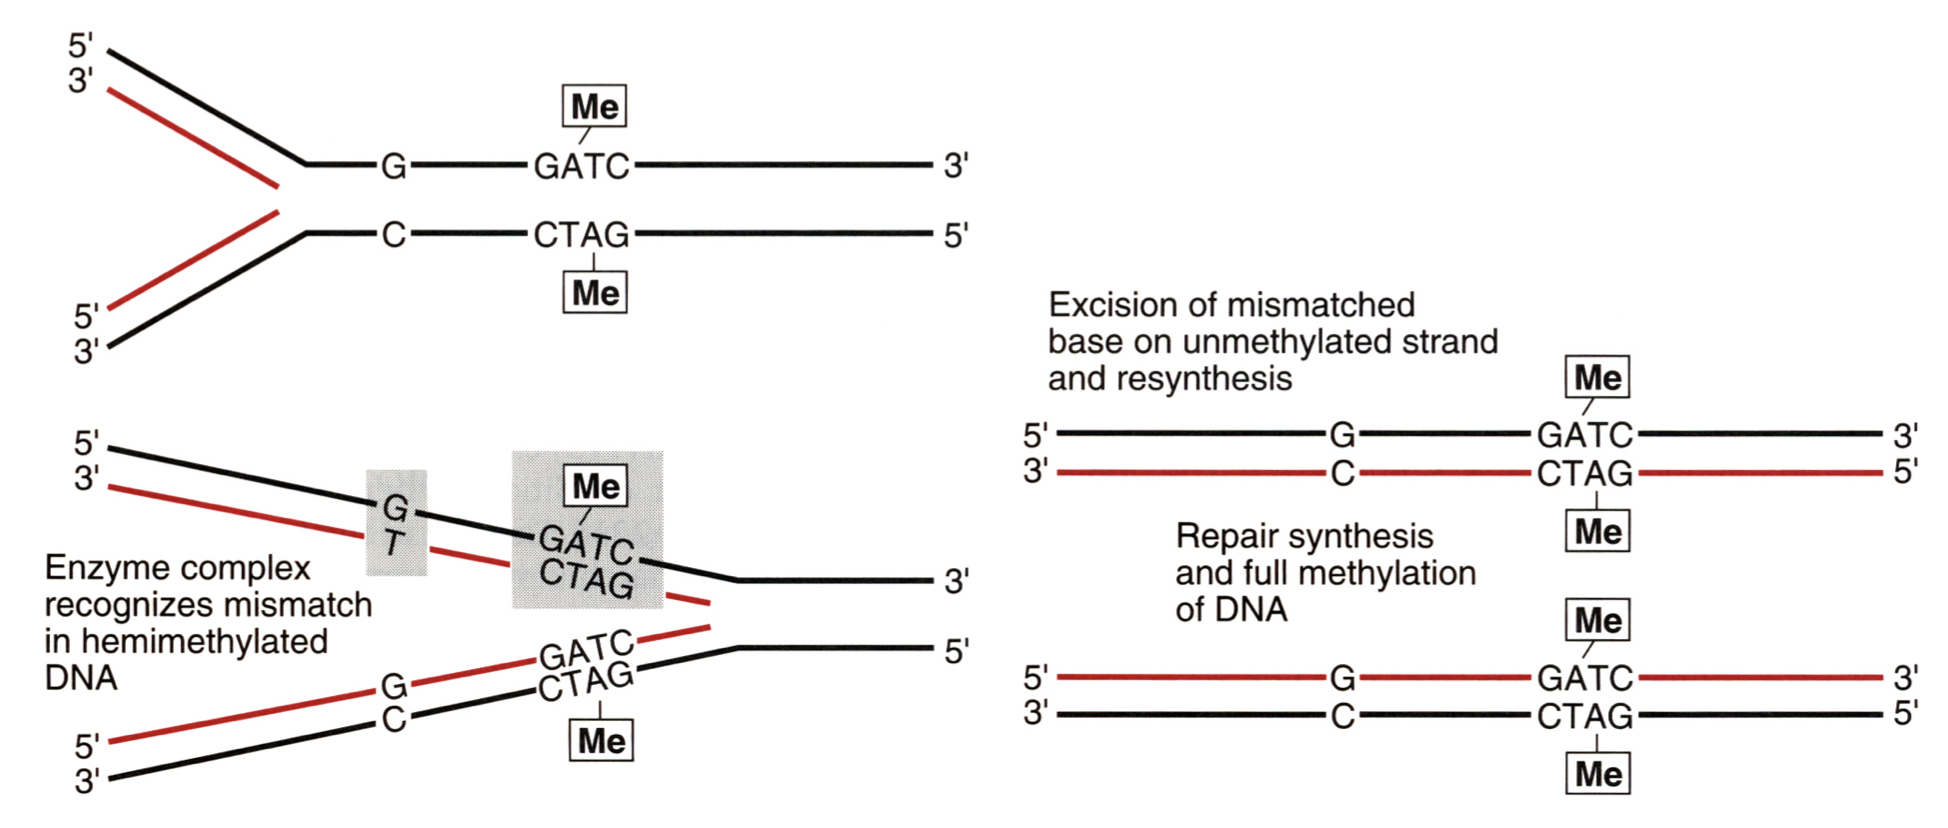
\includegraphics[width=0.9\linewidth]{../ExtFiles/DNARepairc.png}
            \caption{Mismatch repair.}
            \label{fig:DNARepairc}
        \end{subfigure}
        \caption{DNA repair strategies.}
        \label{fig:DNARepair}
    \end{figure}
    \begin{itemize}
        \item Direct reversal/repair (DR): Enzymes catalyze the reverse reaction; no removal or replacement of the base is needed.
        \begin{itemize}
            \item The detailed mechanism of DNA phytolyases is not testable material.
        \end{itemize}
        \item Base excision repair (BER): DNA glycosylases cleave the ribose-base bond to produce apurinic/ apyrimidinic (AP) sites.
        \begin{itemize}
            \item See Figure \ref{fig:DNARepaira}.
            \item Procedure:
            \begin{enumerate}
                \item DNA glycosylases hydrolyze the N-glycosyl bond of damaged bases.
                \item This creates an "AP" site.
                \item AP endonucleases recognize the AP site and hydrolyze the phosphodiester $5'$ or $3'$ of each AP site (mostly $5'$).
                \item Exonucleases remove the backbone at free ends.
                \item DNA polymerase and ligase fill in and seal the gap.
            \end{enumerate}
            \item Most DNA glycosylases recognize a specific damaged base.
            \item In general, $<30$ kD monomeric proteins.
            \item No requirement for cofactors.
        \end{itemize}
        \item Nucleotide excision repair (NER): Enzymes remove a segment of DNA including the lesion and several nucleotides on either side.
        \begin{itemize}
            \item See Figure \ref{fig:DNARepairb}.
            \item Create nicks at two sites. Remove the DNA with lesion. Fill the gap with polymerase. Ligation via ligase.
        \end{itemize}
        \item Mismatch repair (MR): A subset of BER and NER systems that can discriminate an improper base among two normal nucleotides forming a non W-C pair.
        \begin{itemize}
            \item Most repair mechanisms are good for recognizing obvious abnormalities (e.g., uracil in DNA, paired pyrimidines, etc.). MR deals with cases when you have two pairs that don't match and it's not immediately clear which is the error.
            \item Origin of mismatched (non-W-C) natural DNA base pairs:
            \begin{itemize}
                \item DNA polymerase errors: \num{e-4} (intrinsic) $\times$ \num{e-3} (proofreading) = \num{e-7} per base per generation.
                \item Heteroduplex DNA arising from homologous recombination.
                \item Deamination of 5-Me-C to T (forming G:T pairs).
            \end{itemize}
            \item The challenge in repairing a mismatch is distinguishing the "incorrect" base among two natural bases.
            \item Methyl-directed MR.
            \begin{itemize}
                \item See Figure \ref{fig:DNARepairc}.
                \item \emph{E. coli} methylates \ce{N^6} of A in GATC ("dam" methylation).
                \item Methylation lags behind DNA replication (which always makes non-methylated DNA).
                \item 1976: B. Wagner and M. Meselson hypothesized that the lack of methylation in a newly synthesized strand allows strand discrimination during mismatch correction.
            \end{itemize}
            \item Experimental support:
            \begin{itemize}
                \item No PCR, none of today's routine bio experiments were available in the 1980s.
                \item The key experiments: Introduce into cells hemimethylated heteroduplex DNA and allow mismatch repair to take place.
                \item This occurred even if the nearest methylation site was $>1000$ bp from the mismatch!
                \item Neither strand methylated: Correction of either strand.
                \item One strand methylated: Correction of unmethylated strand.
                \item Both strands methylated: Slow correction of either strand.
            \end{itemize}
            \item Current MR model (not testable):
            \begin{itemize}
                \item MutS binds the mismatch or frameshift loop.
                \item MutS/L/H complex brings the mismatch and GATC together.
                \item MutH nicks the nonmethylated strand $5'$ of the GATC.
                \item ExoVII or RecJ degrades $5'$-$3'$ from GATC to the mismatch or Exol degrades $3'$-$5'$ from GATC to the mismatch.
            \end{itemize}
        \end{itemize}
    \end{itemize}
    \item No translation today; will be next time. The next lecture will have less content.
\end{itemize}




\end{document}